\documentclass[12pt]{report}
\usepackage{graphicx}
\usepackage{fancyhdr}
\usepackage{titling}
\usepackage[latin1]{inputenc}
\usepackage{amsmath}
\usepackage{calc}
\usepackage{amssymb}
\usepackage{listings}
\usepackage[usenames]{xcolor}
\usepackage{hyperref}
\hypersetup{
    colorlinks=true,
    linktoc=all,
    linkcolor=black
}

\parindent=0pt
\pagestyle{fancy}

\fancyhead[L]{\slshape\footnotesize November 4, 2013\\\textsc{02249 Computationally Hard Problems}}
\fancyhead[R]{\slshape\footnotesize \textsc{Andreas Kjeldsen (s092638)}\\\textsc{Morten Eskesen (s133304)}}
\fancyfoot[C]{\thepage}

\newcommand{\HRule}{\rule{\linewidth}{0.075mm}}
\newcommand{\HRuleFat}{\rule{\linewidth}{0.5mm}}

\newlength{\depthofsumsign}
\setlength{\depthofsumsign}{\depthof{$\sum$}}
\newcommand{\nsum}[1][1.4]{\mathop{\raisebox{-#1\depthofsumsign+1\depthofsumsign}{\scalebox{#1}{$\displaystyle\sum$}}}}

\begin{document}

\begin{titlepage}
\begin{center}


\includegraphics[scale=2.0]{dtu_logo.pdf}\\[0.70cm]

\textsc{\LARGE Technical University of Denmark}\\[.85cm]

\textsc{\Large 02249 Computationally Hard problems}\\[0.35cm]


% Title
\HRuleFat \\[0.4cm]
{\huge \bfseries Project: Mirror Friendly Minimum Spanning Tree}\\[0.1cm]
\HRuleFat \\[0.4cm]

% Author and supervisor
\large
\emph{Authors:}
\\[10pt]
Andreas Hallberg \textsc{Kjeldsen}\\
\emph{s092638@student.dtu.dk}
\\[10pt]
Morten Chabert \textsc{Eskesen}\\
\emph{s133304@student.dtu.dk}
\\[10pt]

\vfill

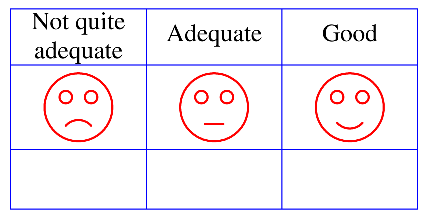
\includegraphics[scale=1]{Evurd.pdf}

% Bottom of the page
{\large November 4, 2013}

\end{center}
\end{titlepage}

\tableofcontents

\chapter{Introduction}
\label{chapt:intro}
This report will focus on a problem called \textsc{MirrorFriendlyMinimumSpanningTree} or $MFMST$ for short. We will present the problem in colloquial terms, show that the problem is in NP and that it is NP-complete. We have also present an algorithm for solving the optimization version of the problem, while providing a description of the algorithm and proving it's worst-case running time.\\
\HRule\\
\textbf{Problem:} \textsc{[MirrorFriendlyMinimumSpanningTree (MFMST)]}\\
\textbf{Input:} An undirected, connected weighted graph $G = (V,E,w)$, where $V = \{1,\dots,n\}$, $E = \{e_1,\dots,e_m\}$ and $w : E \rightarrow \mathbb{N}_0$, and a number $B \in \mathbb{N}$.\\
\textbf{Output:} YES if there is a spanning tree $T \subseteq E$ for $G$ such that
$$max \left\{\nsum\limits_{e_i \in T} w(e_i), \nsum\limits_{e_i \in T} w(e_{m+1-i})\right\} \leq B$$
and NO otherwise.\\
\HRule

\chapter{NP Problems}
\section{Description of the problem in colloquial terms}
A minimum spanning tree is a subgraph within an undirected, connected weighted graph that is a tree and connects all the vertices together with a weight less or equal to the weight of every other spanning tree. The main difference between a minimum spanning tree and a mirror friendly minimum spanning tree is the inequality described in Chapter \ref{chapt:intro}. In a mirror friendly minimum spanning tree the inequality must be satisfied. It should be possible to mirror the spanning tree in such a way that the maximum of the spanning tree and the mirrored spanning tree is less than or equal to a fixed value, $B$. This also means that the mirror friendly minimum spanning tree may not be equal to the minimum spanning tree in the graph, i.e. it may have a larger weight than the minimum spanning tree.

\subsection{Solve an example problem}
\textbf{Input:} $V = \{1,2,3\}$, $E = \{e_1 = \{1,2\},e_2 = \{2,3\},e_3 = \{1,3\}\}$, $w(e_i) = i$ for $i \in \{1,2,3\}$ and $B = 4$.
\begin{center}
\begin{tabular}{ l c c c }
\# & Spanning Tree & & Mirrored Spanning Tree\\
1. & $w(e_1) + w(e_2) = 3$ & & $w(e_{3+1-1)} + w(e_{3+1-2}) = w(e_3) + w(e_2) = 5$\\
2. & $w(e_3) + w(e_1) = 4$ & & $w(e_{3+1-3}) + w(e_{3+1-1}) = w(e_3) + w(e_1) = 4$\\
\end{tabular}
\end{center}
Shown above are the sum of the weights for two pairs of spanning trees. The first pair has a spanning tree with a weight of 3 and a mirrored spanning tree with a weight of 5. The maximum of these values would therefore be 5 which is more than $B$. Therefore the first pair does not satisfy the requirement to be a $MFMST$.
$$max\{3,5\} \leq B \rightarrow 5 \nleq 4$$
The second pair has a spanning tree with a weight of 4 and a mirrored spanning tree with a weight of 4. The maximum of these values would therefore be 4 which is the same as B. The pair therefore satisfies the requirement to be a $MFMST$.
$$max\{4,4\} \leq B \rightarrow 4 \leq 4$$
The algorithm would output YES.

\subsection{Show that MFMST is in $NP$}
\HRule
\begin{center}
\textbf{\textcolor{red}{MINDER DET HER IKKE MEGET OM SLIDES?}}
\end{center}
\HRule
\subsubsection{1. Design a deterministic algorithm $A$ which takes as input a problem instance $X$ and random sequence $R$}

\textbf{Specify what the random sequence $R$ consists of}\\
Let the string $R$ consist of bits: $R = r_1,r_2,\dots,r_n$.\\

\textbf{Specify how $A$ interprets $R$ as a guess}\\
Consider the first $m$ bits. If the $i^{th}$ bit is 1, mark the edge $e_i$.\\

\textbf{Specify how $A$ verifies the guess}\\
If the marked edges create a mirror friendly minimum spanning tree with a weight less than or equal to $B$, answer YES, otherwise NO.

\subsubsection{2. Show that the two conditions are met}
\textbf{\textcolor{red}{$\uparrow$ Skal have en anden titel - M{\aa}ske det skal skrives om til at v{\ae}re med vores eget sprog? Carsten kan jo ikke lide n{\aa}r man er for korrekt.}}\\
\textbf{If true the answer to $X$ is YES, then there is a string $R^*$ with positive probability such that $A(X, R^*) = YES$}
\begin{itemize}
	\item[] Asssume that the answer is YES
	
	\item[] Then there is a subset of the edges that creates a mirror friendly minimum spanning tree with a weight less than or equal to $B$.
	
	\item[] Let $S \subseteq \{1,\dots,m\}$ be the set that describe the edges' index
	
	\item[] Construct the bit string $R^* = r_1,r_2,\dots,r_m$ where $r_i = 1$ if and if only if $i \in S$
	
	\item[] When $A$ receives $R^*$, it will select the edges in $S$, verify that the edges form a spanning tree and that the weight of the edges are less than or equal to $B$ and answer YES.
	
	\item[] Altogether there is a string of length at most $p(n)$ that will give YES. The probability of randomly creating it is positive.
\end{itemize}

\textbf{If true the answer to $X$ is NO, then $A(X, R) = NO$ for all $R$}
\begin{itemize}
	\item[] Assume that the answer is NO
	
	\item[] Then no set of the edges create a mirror friendly minimum spanning tree with a weight less than or equal to $B$.
	
	\item[] If $R$ does not contain enough bits, the algorithm will correctly answer NO.
	
	\item[] Otherwise the algorithm will mark some edges and compute their weight. This will be compared to $B$. But as no set of edges has a weight less than or equal to $B$, the answer is NO.
\end{itemize}

\subsubsection{3. Show that $A$ is $p$-bounded for some polynomial $p$}
\begin{itemize}
	\item[] There are $m$ edges.
	
	\item[] It is checked that the string $R$ consists of at least $m$ bits. Time: $O(m)$.
	
	\item[] Every edge is marked or not marked. Time: $O(m)$.
	
	\item[] The weights of the marked edges are added. Time: $O(m)$.
	
	\item[] The computed total weight is compared to $B$ and the answer is returned. Time: $O(1)$.
\end{itemize}

Altogether the time is: $O(m)$.

\section{Show that MFMST is $NP$-complete}
\subsection{Suitable problem $P_c$ known to be $NP$-complete}
\subsubsection{Select a suitable problem $P_c$ known to be $NP$-complete}
We have chosen to use the problem \textsc{1-In-3-Satisfiability} as our problem $P_c$ which is known to be $NP$-complete.\\
\HRule\\
\textbf{Problem:} \textsc{[1-In-3-Satisfiability]}\\
\textbf{Input:} A set of clauses $C = \{c_1,\dots,c_k\}$ over $n$ boolean variables $x_1,\dots,x_n$, where every clause contains exactly three literals.\\
\textbf{Output:} YES if there is a satisfying assignment such that every clause has exactly one true literal, i.e., if there is an assignment
$$a: \{x_1,\dots,x_n\} \rightarrow \{0,1\}$$
such that every clause $c_j$ is satisfied and no clause has two or three satisfied literals, and NO otherwise.\\
\HRule

\subsubsection{Prove that MFMST is reducable from problem $P_c$}
We wish to prove $$\textsc{1-In-3-Satisfiability} \leq_p \textsc{MirrorFriendlyMinimumSpanningTree}$$

In order to prove this we use component design. When given an instance $(X,C)$ of \textsc{1-In-3-Satisfiability} we construct an instance $(G = (V, E,w),B)$ of MFMST. This is done by building small "component" graphs that are later connected to form the desired graph $G$. The components will have different "responsibilities". Some ensure a correct setting of the truth values, others which test satisfiability and components to connect them.

\subsubsection{Outline of the transformation}
Let $X = \{x_1,\dots,x_n\}$ be the boolean variables and $C = \{c_1,\dots,c_m\}$ the clauses over $X$. We set $B = n + 2m$ for the MFMST instance. We set $w(e_i) = i$. The vertex set of $G$ \textcolor{red}{Maaske skal $a()$ defineres lidt foer, jeg sad og fattede ingenting, samme for $v()$}:
$$V = \{x_1,\dots,x_n\} \cup \{\overline{x}_1,\dots,\overline{x}_n\} \cup \bigcup_{j=1}^{m}{\left\{a_1(j),a_2(j),a_3(j)\right\}}$$

The truth setting components are defined to be the edges.
\begin{center}
	$\forall x_1 \in X$ let $T_1$ be the vertex with incoming edges $x_1$ and $\overline{x}_1$
\end{center}
These components ensure that every spanning tree has to contain at least one of the edges $x_1$ or $\overline{x}_1$.\\
\\
The components for clause satisfiability are defined by the following.
\begin{center}
	$\forall c_j \in C$: let $S_j$ be the set of vertices\\
	$S_j  = \{v_1(j),v_2(j),v_3(j)\}$
\end{center}
Two edges per triangle are needed to make a spanning tree. The edge not chosen is the \emph{true} literal which satisfies $c_j$.\\
\\
The connecting components are defined by the following. Let $c_j = l_1 \vee l_2 \vee l_3$ where $l_k$ are literals. More specifically $l_k$ is a boolean variable $x_i$ or negated boolean variable $\overline{x}_i$. For every clause $c_j$ the following three vertices are added.
$$K_j = \{(v_1(j) \vee l_1), (v_2(j) \vee l_2), (v_3(j) \vee l_3)\}$$

The vertex set $V$ is therefore:
$$V = \bigcup_{i=1}^{n}{T_i} \cup \bigcup_{j=1}^{m}{S_j} \cup \bigcup_{j=1}^{m}{K_j}$$
The transformation $T$ can be performed in time polynomial in $n$ and $m$.

\subsubsection{Answer to $X$ is YES then answer to $T(X)$ is YES}
Assume that $a: X \rightarrow \{0,1\}$ is an assignment which satisfies all clauses $c_j$. Consider the graph $G = (V,E,w)$ constructed above. We begin to construct $T \subseteq E$ by selecting $n$ edges as follows:
$$x_i \in T \Leftrightarrow a(x_i) = 1$$
$$\overline{x}_i \in T \Leftrightarrow a(x_i) = 0$$

Then all $T_i$ are covered. For every clause $c_j$ at least one connecting vertex is covered by an $l_k$ (by virtue of some literal in $c_j$ is set to 1). Assume that for clause $c_j$ this is $l_1$. We add $a_2(j)$ and $a_3(j)$ to $T$. These two edges cover the other two connecting vertices and the three vertices of the triangle $S_j$. The set $T$ is a spanning tree and has weight $B = n + 2m$.

\subsubsection{Answer to $T(X)$ is YES then answer to $X$ is YES}
Lets assume that $T \subseteq E$ is a spanning tree for $G$ with a mirrored spanning tree where both have a weight less than or equal to $B$. In order to cover the vertices at least one of the edges $x_i$ or $\overline{x}_i$ has to be in $T$. In order to cover the vertices of $S_j$, the spanning tree $T$ has to contain at least two of the edges. Therefore $|T| = B = n + 2m$, and we have that $T$ contains exactly one edge from every $T_i$ and exactly two edge from every $S_j$.\\
We define an assignment: $a(x_i) =$ 1 if $x_i \in T$ and 0 if $\overline{x}_i \in T$\\
As $T$ contains exactly one of $x_i$ or $\overline{x}_i$ the assignment $a$ is well defined. We still need to show that the assignment satisfies all clauses $c_j$. Let $c_j = l_1 \vee l_2 \vee l_3$ be a clause where $l_k$ are literals. For every component $S_j$ exactly two edges belong to $T$, say $\{v_1(j),v_2(j)\}$ and $\{v_2(j),v_3(j)\}$. They cover also the connecting vertices $(v_1(j) \vee l_1)$ and $(v_2(j) \vee l_2)$. The third connecting vertex $(v_3(j) \vee l_3)$ attached to $S_j$ has to be covered by $l_3$. By the construction of $G$ $l_3$ corresponds to a literal in $c_j$ and by the construction of the assignment $a$, $l_3$ is set to true and clause $c_j$ is then satisfied because only one literal in a clause must be true.

\chapter{Algorithm}
\section{Find an algorithm which solves the optimizing version of the problem}
\label{sec:alg1}
There are several algorithms for solving the \textsc{Minimum Spanning Tree} problem.  Kruskals, Prims and Chazelles to name a few. We've chosen to use Prims method that uses an \emph{Indexed Minimum Priority Queue}, to keep track of which edge to check next. The algorithm also makes sure not to visit edges twice.\\
The problem we have to solve isn't solved solely by using Prims algorithm. Prims algorithm only finds the actual MST, however we need to find a mirror friendly MST, therefore we had to make modifications to the algorithm.\\
\\
Most noticable changes to the algorithm:
\begin{enumerate}
	\item[] \textbf{Mirror Weight} can now be calculated for a given MST.
	\item[] \textbf{Search using exclusions} of edges to use. We have to exclude some edges to not always find the same MST.
	\item[] \textbf{Mark edges as required} before trying to find the MST.
\end{enumerate}

\subsection{Life of the algorithm}
Here we will describe the lifecycle of the algorithm.
\begin{description}
	\item[Birth] The algorithm is initialized with $G$ the undirected, connected weighted graph. All required fields are set to be of the minimum required size, which is equal to the amount of vertices in $G$ $(|V|)$.
	
	\item[Preschool] The algorithm starts with no initial knowledge, so to start off it finds the MST. With the knowledge of the MST at hand, the mirrored weight of the MST can be calculated. Whichever weight is highest is used as the current \emph{threshold} value. The threshold value will never increase. The algorithm uses a priority queue to prioritize which edges to look at, lowest weight first.
	
	\item[Highschool] The algorithm now has enough knowledge to start exploring the graph in different ways. To make sure the same MST isn't found again, a set is created with the edges in the MST, but edges that are required to form a spanning tree are removed from the set. A powerset of the remaining edges are created. Each set in the powerset is then used to indicate which edges to exclude when performing a new search. Now try to find a MST using each and every exclusion included in the powerset.
	
	\item[University] The algorithm was able to bruteforce a solution, but we want to make it smarter. To enhance the algorithm we have to limit the amount of exclusion sets to check. This is done by using some simple heuristics. If the current exclusion results in a MST not being found then the set of edges in the exclusion should never be tried again, we therefore add the set to a set of sets never to check again. From now on we skip every exclusion set found that is a superset of or equal to any of the sets never to check again. Earlier we specified that the threshold would never increase, but it will in fact decrease. While finding new MSTs using the exclusion sets, the threshold value will be updated if the maximum value of the weight and mirror weight is below the current threshold. The threshold value would be set to the maximum of the weight and the mirror weight, also the MST will be remembered.
	
	\item[Working 9-5] The algorithm still could run better, so instead of overdoing it's workload, it could minimize it even further. When the threshold value is not to be updated, we could check if it is so high that whatever set is the current set to be excluded could be used as a permanent exclusion. In the case that the minimum value of the weight and the mirror weight is equal to or larger than the current threshold value, we then choose to add the exclusion to the set of sets never to check again.
	
	\item[Retirement] At last the algorithm solves the problem. Though it has aged quite a bit and with age comes various defects, one of which could be the ability to sort things properly. Therefore it could be an advantage to avoid looking through the powerset of exclusions based on weight in a sorted fashion, but simply pick them in a random order. Even with a life worth of knowledge it is uncertain which way would be the optimal, a sort based search or random picking based search.
	
	\item[Termination] One may be lucky enough to end their days when their time is due, others unfortunately terminate prematurely due to various factors, in this case one factor could be the allowed running time. Either way, the algorithm will return the spanning tree currently marked as the best MFMST along with the threshold value.
\end{description}


\section{Prove the worst-case running time of the algorithm}
We've outlined the aspects of our algorithm. Now on to the running time.\\
The core part of the algorithm is finding the MST within the current graph excluding the edges specified as the current exclusion.\\
For every MST exploration the algorithm must:
\begin{enumerate}
	\item Create three arrays of size $|V|$. One of the arrays must have specified all it's values, which is a $O(|V|)$ operation.
	\item Empty the priority queue. For each item removed from the queue a call to the $Visit$ method is made. Each vertex can be added at most once, therefore there will be $|V|$ calls to $Visit$.
	\item Make one deletion and one insert/change operation on the priority queue per call to $Visit$. The priority queue has $O(log_2 |V|)$ insertion, change and deletion.
	\item Calculate the weight and mirror weight, both of these action take $O(|E|)$.
	\item Check the threshold value and maybe update the threshold value or add an exclusion to the never check again set, we claim these actions over the long run executes in constant time $O(1)$.
\end{enumerate}
So to sum up, for every MST exploration the running time will be
$$O(|V| + |V|*(log_2 |V|) + |E|)$$
\\
After the initial MST is found, the required edges can be calculated, this takes $O(|E|)$.\\
\\
Now on to the powerset of exclusions. For any set of size $n$, the powerset of that set will contain $2^n$ subsets (including the empty set). So in our worst-case the set of exclusions to try would be of size $2^{|E|}$. For every exclusion in the powerset we have to run the MST exploration. The generation of each subset of the powerset is assumed to be done in constant time $O(1)$.\\
\\
Putting all this together gives us the following running time:
$$O(2^{|E|}*(|V| + |V|*(log_2 |V|) + |E|) + |E|) \Rightarrow O(2^{|E|})$$

Our algorithm has a polynomial bound worst-case running time of $O(2^{|E|})$.

\chapter{Implementation}
\section{Implement the algorithm developed in \ref{sec:alg1}}
We have chosen to make our implementation in C\#. We've included our .NET Solution in the zip.
\subsection{Running the program}
The program can be run in two ways.
\begin{enumerate}
	\item MFMSTProject.exe [max\_execution\_time] $<$ input.file
	\item MFMSTProject.exe input.file [max\_executation\_time]
\end{enumerate}

For both, the [max\_execution\_time] is an optional parameter stating how many milliseconds the program may use in trying to find the MFMST. If none is set, the default is 20000 milliseconds as per requirement for the contest. If no input.file is specified it will look for a file with the following relative path: $TestFiles/test03.uwg$.
\newpage
\subsection{Example run}
\begin{lstlisting}[basicstyle=\footnotesize]
	MFMSTProject.exe < TestFiles/test03.uwg
	
	Time taken: 187 ms
	Solution:
	Edge 1: {1, 2}; weight: 50, mirrored weight: 51
	Edge 2: {2, 3}; weight: 88, mirrored weight: 13
	Edge 3: {3, 4}; weight: 66, mirrored weight: 10
	Edge 5: {5, 6}; weight: 77, mirrored weight: 14
	Edge 6: {6, 7}; weight: 3, mirrored weight: 52
	Edge 7: {7, 8}; weight: 7, mirrored weight: 61
	Edge 8: {8, 9}; weight: 18, mirrored weight: 38
	Edge 9: {9, 10}; weight: 84, mirrored weight: 69
	Edge 10: {10, 11}; weight: 45, mirrored weight: 61
	Edge 13: {13, 14}; weight: 53, mirrored weight: 75
	Edge 14: {14, 15}; weight: 5, mirrored weight: 4
	Edge 15: {15, 16}; weight: 17, mirrored weight: 20
	Edge 16: {16, 17}; weight: 73, mirrored weight: 57
	Edge 17: {17, 18}; weight: 17, mirrored weight: 33
	Edge 18: {18, 19}; weight: 57, mirrored weight: 7
	Edge 19: {19, 20}; weight: 7, mirrored weight: 49
	Edge 20: {20, 21}; weight: 49, mirrored weight: 7
	Edge 21: {21, 22}; weight: 7, mirrored weight: 57
	Edge 22: {22, 23}; weight: 33, mirrored weight: 17
	Edge 24: {24, 25}; weight: 20, mirrored weight: 17
	Edge 25: {25, 26}; weight: 4, mirrored weight: 5
	Edge 29: {29, 30}; weight: 61, mirrored weight: 45
	Edge 31: {2, 10}; weight: 38, mirrored weight: 18
	Edge 32: {4, 12}; weight: 61, mirrored weight: 7
	Edge 33: {5, 13}; weight: 52, mirrored weight: 3
	Edge 34: {18, 25}; weight: 14, mirrored weight: 77
	Edge 36: {20, 27}; weight: 10, mirrored weight: 66
	Edge 37: {21, 28}; weight: 13, mirrored weight: 88
	Edge 38: {22, 29}; weight: 51, mirrored weight: 50
	
	Solution value: 1080 / 1071
\end{lstlisting}


\end{document}
